\documentclass[CJK,13pt]{beamer}
\usepackage{CJKutf8}
\usepackage{beamerthemesplit}
\usetheme{Malmoe}
\useoutertheme[footline=authortitle]{miniframes}
\usepackage{amsmath}
\usepackage{amssymb}
\usepackage{graphicx}
\usepackage{eufrak}
\usepackage{color}
\usepackage{slashed}
\usepackage{simplewick}
\usepackage{tikz}
\usepackage{tcolorbox}
\usepackage{ulem}
\graphicspath{{../figures/}}
%%figures
\def\lfig#1#2{\includegraphics[width=#1 in]{#2}}
\def\tfig#1#2{\includegraphics[height=#1 in]{#2}}
\def\addfig#1#2{\begin{center}\includegraphics[width=#1 in]{#2}\end{center}}
\def\question{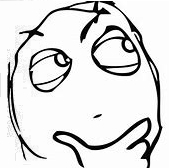
\includegraphics[width=0.3in]{why.jpg}\,}
\def\answer{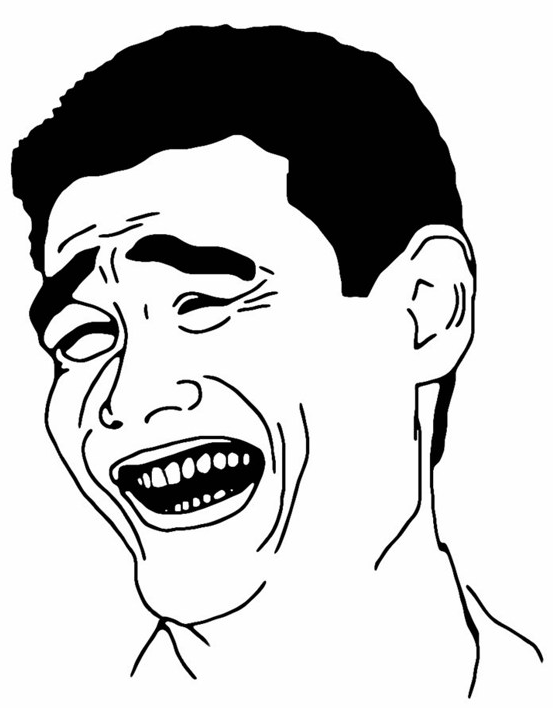
\includegraphics[width=0.3in]{baozou_haha.png}\,}
\def\wulian{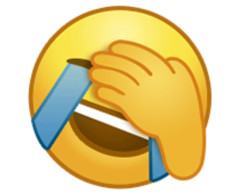
\includegraphics[width=0.18in]{emoji_wulian.jpg}}
\def\bigwulian{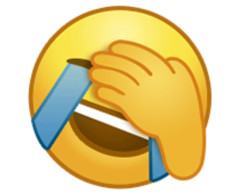
\includegraphics[width=0.35in]{emoji_wulian.jpg}}
\def\bye{
\includegraphics[width=0.18in]{emoji_bye.jpg}}
\def\bigbye{
\includegraphics[width=0.35in]{emoji_bye.jpg}}
\def\huaixiao{
\includegraphics[width=0.18in]{emoji_huaixiao.jpg}}
\def\bighuaixiao{
\includegraphics[width=0.35in]{emoji_huaixiao.jpg}}
\def\jianxiao{
\includegraphics[width=0.18in]{emoji_jianxiao.jpg}}
\def\bigjianxiao{
\includegraphics[width=0.35in]{emoji_jianxiao.jpg}}
\def\haoqi{
\includegraphics[width=0.18in]{emoji_haoqi.jpg}}
%% colors
\def\blacktext#1{{\color{black}#1}}
\def\bluetext#1{{\color{blue}#1}}
\def\redtext#1{{\color{red}#1}}
\def\darkbluetext#1{{\color[rgb]{0,0.2,0.6}#1}}
\def\skybluetext#1{{\color[rgb]{0.2,0.7,1.}#1}}
\def\cyantext#1{{\color[rgb]{0.,0.5,0.5}#1}}
\def\greentext#1{{\color[rgb]{0,0.7,0.1}#1}}
\def\darkgray{\color[rgb]{0.2,0.2,0.2}}
\def\lightgray{\color[rgb]{0.6,0.6,0.6}}
\def\gray{\color[rgb]{0.4,0.4,0.4}}
\def\blue{\color{blue}}
\def\red{\color{red}}
\def\orange{\color[rgb]{1.,0.8,0.}}
\def\green{\color{green}}
\def\darkgreen{\color[rgb]{0,0.4,0.1}}
\def\darkblue{\color[rgb]{0,0.2,0.6}}
\def\skyblue{\color[rgb]{0.2,0.7,1.}}
%%control
\def\diag{\mathrm{diag}\,}
\def\heaviside{\,\mathrm{h}\,}
\def\bral{\left(\begin{array}{l}}
\def\brar{\end{array}\right)}
\def\brall{\left(\begin{array}{ll}}
\def\brarr{\end{array}\right)}
\def\bralll{\left(\begin{array}{lll}}
\def\brarrr{\end{array}\right)}
\def\branchl{\left\{\begin{array}{l}}
\def\branchr{\end{array}\right.}
\def\branchll{\left\{\begin{array}{ll}}
\def\branchrr{\end{array}\right.}
\def\branchlll{\left\{\begin{array}{lll}}
\def\branchrrr{\end{array}\right.}
\def\sfgamma#1{\,\Gamma\left( #1 \right)\,}
\def\be{\begin{equation}}
\def\ee{\nonumber\end{equation}}
\def\bea{\begin{eqnarray}}
\def\eea{\nonumber\end{eqnarray}}
\def\bch{\begin{CJK}{UTF8}{gbsn}}
\def\ech{\end{CJK}}
\def\bitem{\begin{itemize}}
\def\eitem{\end{itemize}}
\def\bcenter{\begin{center}}
\def\ecenter{\end{center}}
\def\bex{\begin{minipage}{0.2\textwidth}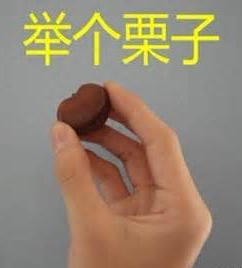
\includegraphics[width=0.6in]{jugelizi.png}\end{minipage}\begin{minipage}{0.76\textwidth}}
\def\eex{\end{minipage}}
\def\chtitle#1{\frametitle{\bch#1\ech}}
\def\bmat#1{\left(\begin{array}{#1}}
\def\emat{\end{array}\right)}
\def\bcase#1{\left\{\begin{array}{#1}}
\def\ecase{\end{array}\right.}
\def\bmini#1{\begin{minipage}{#1\textwidth}}
\def\emini{\end{minipage}}
\def\tbox#1{\begin{tcolorbox}#1\end{tcolorbox}}
\def\pfrac#1#2#3{\left(\frac{\partial #1}{\partial #2}\right)_{#3}}
\def\res#1#2{\,\mathrm{res}\,#1\left(#2\right)\,}
\def\newt#1#2{\left(\begin{array}{c}#1\\ #2\end{array}\right)}
\def\reof#1{\,\mathrm{Re}{\left(#1\right)\,}}
\def\imof#1{\,\mathrm{Im}{\left(#1\right)\,}}
\def\Arg#1{\,\mathrm{Arg}\,#1\,}
%%symbols
\def\intfull{\int_{-\infty}^\infty}
\def\inthalf{\int_0^\infty}
\def\bropt{\,(\ \ \ )}
\def\sech{\mathrm{sech}\,}
\def\csch{\mathrm{csch}\,}
\def\asinh{\mathrm{asinh}\,}
\def\acosh{\mathrm{acosh}\,}
\def\sone{$\star$}
\def\stwo{$\star\star$}
\def\sthree{$\star\star\star$}
\def\sfour{$\star\star\star\star$}
\def\sfive{$\star\star\star\star\star$}
\def\rint{{\int_\leftrightarrow}}
\def\roint{{\oint_\leftrightarrow}}
\def\stdHf{{\textit{\r H}_f}}
\def\deltaH{{\Delta \textit{\r H}}}
\def\ii{{\dot{\imath}}}
\def\skipline{{\vskip0.1in}}
\def\skiplines{{\vskip0.2in}}
\def\lagr{{\mathcal{L}}}
\def\hamil{{\mathcal{H}}}
\def\vecT{{\mathbf{T}}}
\def\vecN{{\mathbf{N}}}
\def\vecB{{\mathbf{B}}}
\def\vecv{{\mathbf{v}}}
\def\vecr{{\mathbf{r}}}
\def\vecf{{\mathbf{f}}}
\def\vecg{{\mathbf{g}}}
\def\vecupsilon{{\mathbf{\upsilon}}}
\def\vecu{{\mathbf{u}}}
\def\vecj{{\mathbf{j}}}
\def\vecx{{\mathbf{x}}}
\def\vecy{{\mathbf{y}}}
\def\vecz{{\mathbf{z}}}
\def\veck{{\mathbf{k}}}
\def\vecp{{\mathbf{p}}}
\def\vecn{{\mathbf{n}}}
\def\vecA{{\mathbf{A}}}
\def\vecP{{\mathbf{P}}}
\def\vecsigma{{\mathbf{\sigma}}}
\def\hatJn{{\hat{J_\vecn}}}
\def\hatJx{{\hat{J_x}}}
\def\hatJy{{\hat{J_y}}}
\def\hatJz{{\hat{J_z}}}
\def\hatj#1{\hat{J_{#1}}}
\def\hatphi{{\hat{\phi}}}
\def\hatq{{\hat{q}}}
\def\hatpi{{\hat{\pi}}}
\def\vel{\upsilon}
\def\Dint{{\mathcal{D}}}
\def\adag{{\hat{a}^\dagger}}
\def\bdag{{\hat{b}^\dagger}}
\def\cdag{{\hat{c}^\dagger}}
\def\ddag{{\hat{d}^\dagger}}
\def\hata{{\hat{a}}}
\def\hatb{{\hat{b}}}
\def\hatc{{\hat{c}}}
\def\hatd{{\hat{d}}}
\def\hatD{{\,\hat{D}}}
\def\hatN{{\hat{N}}}
\def\hatH{{\hat{H}}}
\def\hatp{{\hat{p}}}
\def\Fup{{F^{\mu\nu}}}
\def\Fdown{{F_{\mu\nu}}}
\def\newl{\nonumber \\}
\def\vece{\mathrm{e}}
\def\calM{{\mathcal{M}}}
\def\calT{{\mathcal{T}}}
\def\calR{{\mathcal{R}}}
\def\barpsi{\bar{\psi}}
\def\baru{\bar{u}}
\def\barv{\bar{\upsilon}}
\def\qeq{\stackrel{?}{=}}
\def\ftf{\stackrel{\mathcal{FT}}{\Longrightarrow}}
\def\ftb{\stackrel{\mathcal{FT}}{\Longleftarrow}}
\def\ftfb{\stackrel{\mathcal{FT}}{\Longleftrightarrow}}
\def\ltf{\stackrel{\mathcal{LT}}{\Longrightarrow}}
\def\ltb{\stackrel{\mathcal{LT}}{\Longleftarrow}}
\def\ltfb{\stackrel{\mathcal{LT}}{\Longleftrightarrow}}
\def\torder#1{\mathcal{T}\left(#1\right)}
\def\rorder#1{\mathcal{R}\left(#1\right)}
\def\contr#1#2{\contraction{}{#1}{}{#2}#1#2}
\def\trof#1{\mathrm{Tr}\left(#1\right)}
\def\trace{\mathrm{Tr}}
\def\comm#1{\ \ \ \left(\mathrm{used}\ #1\right)}
\def\tcomm#1{\ \ \ (\text{#1})}
\def\slp{\slashed{p}}
\def\slk{\slashed{k}}
\def\calp{{\mathfrak{p}}}
\def\veccalp{\mathbf{\mathfrak{p}}}
\def\Tthree{T_{\tiny \textcircled{3}}}
\def\pthree{p_{\tiny \textcircled{3}}}
\def\dbar{{\,\mathchar'26\mkern-12mu d}}
\def\erf{\mathrm{erf}}
\def\const{\mathrm{const.}}
\def\pheat{\pfrac p{\ln T}V}
\def\vheat{\pfrac V{\ln T}p}
%%units
\def\fdeg{{^\circ \mathrm{F}}}
\def\cdeg{^\circ \mathrm{C}}
\def\atm{\,\mathrm{atm}}
\def\angstrom{\,\text{\AA}}
\def\SIL{\,\mathrm{L}}
\def\SIkm{\,\mathrm{km}}
\def\SIyr{\,\mathrm{yr}}
\def\SIGyr{\,\mathrm{Gyr}}
\def\SIV{\,\mathrm{V}}
\def\SImV{\,\mathrm{mV}}
\def\SIeV{\,\mathrm{eV}}
\def\SIkeV{\,\mathrm{keV}}
\def\SIMeV{\,\mathrm{MeV}}
\def\SIGeV{\,\mathrm{GeV}}
\def\SIcal{\,\mathrm{cal}}
\def\SIkcal{\,\mathrm{kcal}}
\def\SImol{\,\mathrm{mol}}
\def\SIN{\,\mathrm{N}}
\def\SIHz{\,\mathrm{Hz}}
\def\SIm{\,\mathrm{m}}
\def\SIcm{\,\mathrm{cm}}
\def\SIfm{\,\mathrm{fm}}
\def\SImm{\,\mathrm{mm}}
\def\SInm{\,\mathrm{nm}}
\def\SImum{\,\mathrm{\mu m}}
\def\SIJ{\,\mathrm{J}}
\def\SIW{\,\mathrm{W}}
\def\SIkJ{\,\mathrm{kJ}}
\def\SIs{\,\mathrm{s}}
\def\SIkg{\,\mathrm{kg}}
\def\SIg{\,\mathrm{g}}
\def\SIK{\,\mathrm{K}}
\def\SImmHg{\,\mathrm{mmHg}}
\def\SIPa{\,\mathrm{Pa}}
%page
\def\secpage#1#2{\begin{frame}\bcenter{\bf \Huge #1} \ecenter \skipline \tbox{\bcenter #2 \ecenter}\end{frame}}
\def\append#1#2{\secpage{附录#1}{#2}}
\def\thinka#1{\begin{frame}\frametitle{思考题}\bcenter\lfig{0.4}{think0.jpg}  \skipline #1 \ecenter\end{frame}}
\def\thinkb#1{\begin{frame}\frametitle{思考题}\bcenter\lfig{0.5}{think1.jpg}  \skipline #1 \ecenter\end{frame}}
\def\thinkc#1{\begin{frame}\frametitle{思考题}\bcenter\lfig{0.5}{think2.jpg}  \skipline #1 \ecenter\end{frame}}
\def\thinkd#1{\begin{frame}\frametitle{思考题}\bcenter\lfig{0.5}{think3.jpg}  \skipline #1 \ecenter\end{frame}}
\def\thinke#1{\begin{frame}\frametitle{思考题}\bcenter\lfig{0.5}{think4.jpg}  \skipline #1 \ecenter\end{frame}}
\def\thinkf#1{\begin{frame}\frametitle{思考题}\bcenter\lfig{0.5}{think5.jpg}  \skipline #1 \ecenter\end{frame}}
\def\schw{ds^2 = \left(1-\frac{2GM}{r}\right)dt^2 - \left(1-\frac{2GM}{r}\right)^{-1} dr^2 - r^2\left(d\theta^2 + \sin^2\theta d\phi^2\right)}

\input{titlepage.tex}
  \date{}
  \begin{document}
  \bch
  \tpage{19}{General Discussion about Black Holes}

  \begin{frame}
    我无意在幼儿版GR中把大家拉黑(拉入黑洞知识的泥潭),这一讲的唯一目的是让你不至于在听有关黑洞的讲座时全程梦游。

    \addfig{1.2}{mengyou.jpg}
  \end{frame}


  \secpage{Kerr Black Hole}{    \bea
    ds^2 &=& \left(1-\frac{2GMr}{r^2+a^2\cos^2\theta}\right) dt^2 \newl    
    && + \frac{4GMra\sin^2\theta}{r^2+a^2\cos^2\theta} dt d\phi \newl
    && -\left(r^2+a^2+\frac{2GMra^2\sin^2\theta}{r^2+a^2\cos^2\theta}\right)\sin^2\theta d\phi^2 \newl
    && - \frac{r^2+a^2\cos^2\theta}{r^2-2GMr + a^2}dr^2 \newl
    && - \left(r^2+a^2\cos^2\theta\right)d\theta^2
    \eea
}
  
  \begin{frame}
    \frametitle{Kerr Black Hole}
    黑洞附近的气体和其他天体会被黑洞吞噬,吞噬的过程中黑洞会吸收它们的轨道角动量。所以宇宙中的黑洞应该都或多或少有些“自转”。这种黑洞叫做 Kerr 黑洞。


    \addfig{1}{RealBH.jpg}
  \end{frame}

  \begin{frame}
    如果取其“自转轴”为南北极方向建立“球坐标系”,质量为 $M$,单位质量的角动量为 $a$ 的Kerr黑洞的度规为
{\blue
    \bea
    ds^2 &=& \left(1-\frac{2GMr}{r^2+a^2\cos^2\theta}\right) dt^2 \newl    
    && + \frac{4GMra\sin^2\theta}{r^2+a^2\cos^2\theta} dt d\phi \newl
    && -\left(r^2+a^2+\frac{2GMra^2\sin^2\theta}{r^2+a^2\cos^2\theta}\right)\sin^2\theta d\phi^2 \newl
    && - \frac{r^2+a^2\cos^2\theta}{r^2-2GMr + a^2}dr^2 \newl
    && - \left(r^2+a^2\cos^2\theta\right)d\theta^2
    \eea
}
(哇!五行就写完了!)
  \end{frame}


  \begin{frame}
    \frametitle{因为Kerr度规相关的表达式都太长了,我们要约定一些符号来尽可能地保护视力。}
    \bitem
  \item{定义符号 {\blue $ \rho^2 \equiv r^2+a^2\cos^2\theta $}}
  \item{定义符号 {\blue $ \Delta \equiv r^2-2rGM+a^2 $} ($\Delta$ 是长度平方量纲)}
    \eitem

  \end{frame}


  \begin{frame}
    
    这样Kerr黑洞的度规可以按 $(t, r, \theta,\phi)$ 的坐标次序写为:
    \be
    g_{\mu\nu} = \left[\begin{matrix}    
        1-\frac{2GMr}{\rho^2} &  &  & \frac{2GMra\sin^2\theta}{\rho^2} \\
         & - \frac{\rho^2}{\Delta} &  &  \\
         &  & - \rho^2 &  \\
        \frac{2GMra\sin^2\theta}{\rho^2} &   &  & -\left(r^2+a^2+\frac{2GMra^2\sin^2\theta}{\rho^2}\right)\sin^2\theta 
      \end{matrix}\right]
    \ee
    
  \end{frame}

  \begin{frame}
    \frametitle{逆变形式的度规}

    \be
    g^{\mu\nu} = \left[\begin{matrix}
        \frac{2 GM a^2 r \sin^2\theta   + (r^2+a^2)\rho^2}{  \rho^2\Delta} &  &  & \frac{2 GM a r}{\rho^2\Delta}\\
         & -\frac{\Delta}{\rho^2} &  & \\
         &  & - \frac{1}{\rho^2} & \\
        \frac{2 GM a r}{\rho^2\Delta} &  &  & \frac{2 GM r - \rho^2}{\rho^2\Delta \sin^2\theta }
      \end{matrix}\right]
    \ee

  \end{frame}
  

  \begin{frame}
    \frametitle{Kerr几何}
    \addfig{3.8}{KerrGeometry.png}
  \end{frame}  


  \begin{frame}
    \frametitle{Kerr度规里的测试粒子}
    度规 $g_{\mu\nu}$ 仍然不依赖于 $t$ 和 $\phi$,所以 $p_t$ 和 $p_\phi$ 守恒。

    \skipline
    
    此外,$ds^2$ 表达式照例会给我们一个方程。

    \skipline
    
    由于失去了空间对称性,{\blue 不能再假设测试粒子在一个平面上运动}(除非刚好粒子位置和初速度都在赤道平面 $\theta=\frac{\pi}{2}$ 上)。

    \skipline
    
    还缺的一个方程只能用最原始的测地线方程来凑。

    \skipline
    
    为此我们要计算联络……


  \end{frame}
  

  \begin{frame}
    \addfig{3.8}{Kerrconn.png}
  \end{frame}


  \begin{frame}
    虽然完全算不动,但是为了能吹几句——
  \end{frame}


  \begin{frame}
    \frametitle{引力拖曳效应}
    在赤道( $\theta=\frac{\pi}{2}$) 平面上运动的粒子,$p_\phi$ 守恒可以写成:
    $$ -\frac{2GMa}{r}\frac{dt}{ds}+\left(r^2+a^2+\frac{2GMa^2}{r}\right)\frac{d\phi}{ds} = \frac{L}{m}$$    
    考虑一个非常简化的情形,$r\gg GM \gg a $,且粒子运动速度远小于光速。也就是说,Kerr黑洞的角动量比较小,且测试粒子离得比较远,运动是非相对论的。这时取最低阶近似,有
    $$ \frac{d\phi}{dt} \approx \frac{\frac{L}{m}+\frac{2GMa}{r}}{r^2+a^2}$$
    可以看到,即使粒子的守恒角动量为零(比如它从很远处瞄准黑洞中心下落过来),它也会被黑洞的自旋带着旋转起来,旋转方向和黑洞自旋方向一致。这就是引力拖曳效应。
  \end{frame}
  
  \begin{frame}
    \frametitle{$a>GM$的Kerr度规存在吗?}
    物理学家们猜想有一条“宇宙监督”(cosmic censorship) 法则,使得所有的奇点都被保护在视界之内。

    \skipline
    
    当 $a>GM$ Kerr度规的奇点就会失去视界的“保护”。这种时空“很难”(因为不好严格证明,所以只能这么说)形成,因为当单位质量角动量过大时,物质不容易掉进黑洞。所以至少定性地说,“宇宙监督法则”是有些根据的猜测。
  \end{frame}  


    \begin{frame}
      \frametitle{带电的黑洞}
      稳态的黑洞除了质量,角动量,原则上来讲还可以有电荷$Q$ (即所谓的稳态黑洞只有三个参数的“无毛定理”)。

      这时只要把Kerr度规的
      $$\Delta \equiv r^2+a^2-2GMr$$
      换为
      $$\Delta \equiv r^2+a^2-2GMr+GQ^2$$
      这样得到的度规称为 Kerr-Newman 度规。它是最一般的稳定黑洞。


      \skipline

      相关知识可以参考

      \url{https://arxiv.org/pdf/1410.6626.pdf}
  \end{frame}  

    \secpage{黑洞辐射}{$$ T = \frac{\hbar c^3}{4k_BGM} $$}
    
    \begin{frame}
      我们来估算下质量为 $M$ 的史瓦西黑洞的“视界温度”:黑洞把粒子禁锢在 $\Delta t\sim \frac{4\pi GM}{c^3}$ 大小的时间区域内(注意 $r<2GM$ 时,$r$ 是类时坐标),根据海森堡不确定原理,黑洞视界内的粒子满足
      $$\Delta E \Delta t \gtrsim \frac{\hbar}{2}$$
      于是可以估算出粒子能量的量子波动
      $$\Delta E \sim \frac{\hbar c^3}{8\pi GM}$$
      那么史瓦西黑洞的``温度''
      $$T \sim \frac{\Delta E}{k_B} \sim \frac{\hbar c^3}{8\pi k_BGM}$$      
      ……好了这种瞎扯实在太不严肃,我编不下去了。
    \end{frame}

    \begin{frame}
      \frametitle{正经的结论}
      史瓦西黑洞的“霍金温度”
      {\blue $$ T = \frac{\hbar c^3}{8\pi k_BGM} $$}
      严肃的证明要在很厚的书里才能找到,我们幼儿版GR直接略去……

      \skipline
      
      简单估算一下,太阳质量黑洞的霍金温度大约为 $4\times 10^{-7}\mathrm{K}$,好像完全可以忽略。

      但是,小质量黑洞的霍金温度就会更高,由此产生的辐射会使小质量黑洞逐渐损失质量,这就是“黑洞蒸发”效应。
    \end{frame}

    \begin{frame}
      \frametitle{史瓦西黑洞的辐射功率}
      回忆一下黑体单位表面积的辐射功率为:
      $$\frac{dP}{dS} = \frac{\pi^2k_B^4}{60\hbar^3c^2} T^4$$
      贯彻我们的瞎扯精神,把黑洞当成黑体(反正就差一个字\lfig{0.2}{emoji_wulian.jpg}),把黑洞视界当成“表面”,史瓦西黑洞的辐射功率为:
      $$ P =  4\pi \left(\frac{2GM}{c^2}\right)^2 \frac{\pi^2k_B^4}{60\hbar^3c^2}  \left(\frac{\hbar c^3}{8\pi k_BGM}\right)^4 =\frac{c^6\hbar}{15360\pi G^2M^2}$$
      虽然推导是瞎编的,但是结论仍然正确:
      {\blue $$P = \frac{c^6\hbar}{15360\pi G^2M^2}$$}
    \end{frame}

    \begin{frame}
      \frametitle{史瓦西黑洞的蒸发}
      我们继续按照“能量守恒”编出下列史瓦西黑洞的蒸发公式:
      $$\frac{d\left(Mc^2\right)}{dt} = -P = - \frac{c^6\hbar}{15360\pi G^2M^2}$$
      这里的 $t$ 是史瓦西坐标系里的 $t$,也就是无穷远处相对于坐标系静止的观测者的固有时间。

      把蒸发公式等价地写成:
      $$\frac{d(M^3)}{dt} = -P = - \frac{c^4\hbar}{5120\pi G^2}$$
      可见质量为 $M$ 的史瓦西黑洞的寿命为
     {\blue $$t = \frac{5120\pi G^2M^3}{c^4\hbar}$$}      
    \end{frame}


    \begin{frame}
      \frametitle{原初黑洞的质量下限}
      把黑洞寿命等价地写成:
      $$\frac{t}{\mathrm{Gyr}} = 2.67 \left(\frac{M}{10^{11}\mathrm{kg}}\right)^3 $$
      这里的 $\mathrm{Gyr}$ 是 $10^9$ 年。

      \skiplines

      如果按照标准宇宙学模型的观点,宇宙的年龄大概是 $13.7\mathrm{Gyr}$。那么我们能看到的来自宇宙早期的史瓦西黑洞就有个$\sim 10^{11}\mathrm{kg}$ 的质量下限。
    \end{frame}    
    

    \ech
\end{document}




  
